\begin{figure*}
    \centering
    \begin{subfigure}{\textwidth}
    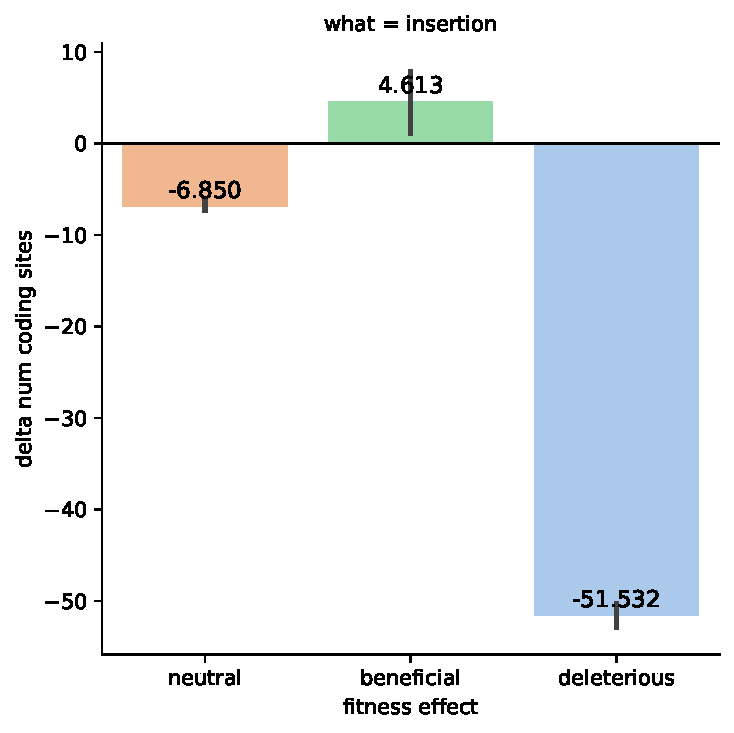
\includegraphics[width=0.5\linewidth]{binder/binder/teeplots/col=what+hue=fitness-effect+kind=bar+palette=pastel+textlabels=True+viz=catplot+x=fitness-effect+y=delta-num-coding-sites+ext=.pdf}%
    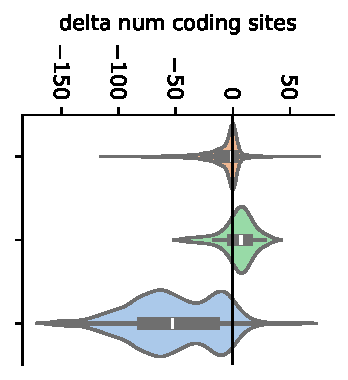
\includegraphics[width=0.5\textwidth]{binder/binder/teeplots/col=what+hue=fitness-effect+kind=violin+palette=pastel+textlabels=True+viz=catplot+x=fitness-effect+y=delta-num-coding-sites+ext=.pdf}

    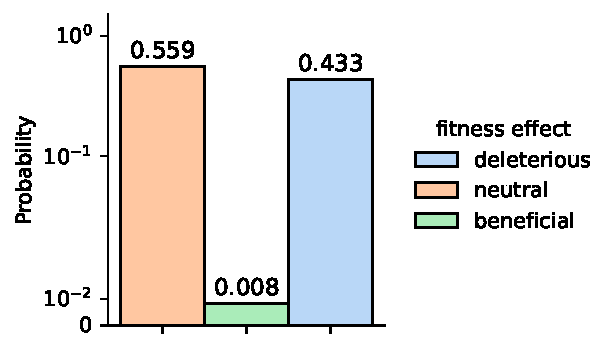
\includegraphics[width=0.5\linewidth]{binder/binder/teeplots/col=what+hue=fitness-effect+kind=hist+multiple=stack+palette=pastel+stat=probability+viz=displot+x=fitness-effect+ext=.pdf}

    \caption{\footnotesize aggregated over lineage histories}
    \end{subfigure}

    \begin{subfigure}{\textwidth}
    \centering
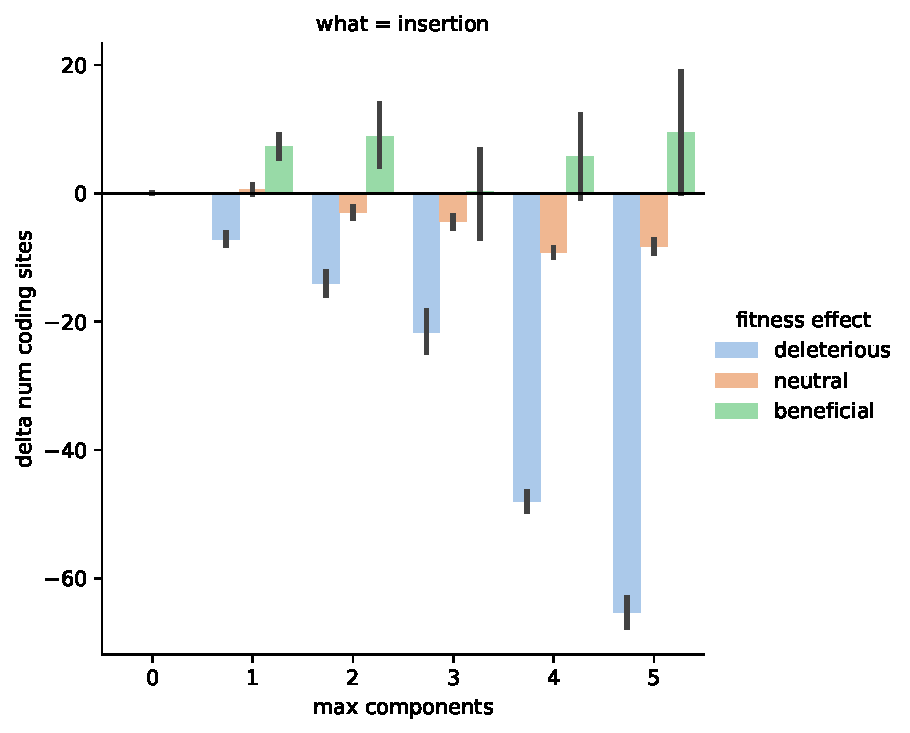
\includegraphics[width=0.5\linewidth]{binder/binder/teeplots/col=what+hue=fitness-effect+kind=bar+palette=pastel+viz=catplot+x=max-components+y=delta-num-coding-sites+ext=.pdf}
    \caption{\footnotesize split by genome task complexity}
    \end{subfigure}
    \caption{
        \textbf{Null distribution of insertion mutation outcomes, sampled over slip-duplication treatment lineage histories.}
        \footnotesize
        Notably, insertion mutations that neither add or lose tasks tend to decrease brittleness, reducing the number of task-critical coding sites --- particularly for genomes that have acquired complex tasks.
        Unsurprisingly, deleterious mutations tend to greatly decrease coding site count and beneficial mutations, which add new tasks, tend to increase them.
        Error bars give bootstrapped 95\% CI.
    }
    \label{fig:nulldist}
\end{figure*}
